% Created 2011-11-26 sam. 12:45
\documentclass[11pt]{article}
\usepackage[utf8]{inputenc}
\usepackage[T1]{fontenc}
\usepackage{fixltx2e}
\usepackage{graphicx}
\usepackage{longtable}
\usepackage{float}
\usepackage{wrapfig}
\usepackage{soul}
\usepackage{textcomp}
\usepackage{marvosym}
\usepackage{wasysym}
\usepackage{latexsym}
\usepackage{amssymb}
\usepackage{hyperref}
\tolerance=1000
\usepackage{minted}
\usepackage[french]{babel}
\usepackage{hyperref}
\hypersetup{colorlinks=true,urlcolor=blue,linkcolor=blue,}
\usepackage{geometry}
\geometry{left=1.2in,right=1.2in,top=1.2in,bottom=1.2in}
\providecommand{\alert}[1]{\textbf{#1}}

\title{ONE LAPTOP PER CHILD\\GUIDE DE DEPLOIEMENT 2011}
\author{OLPC Foundation (c) 2011 One Laptop Per Child Association, Inc.\\Traduction OLPC France}
\date{Novembre 2011}
\hypersetup{
  pdfkeywords={},
  pdfsubject={},
  pdfcreator={Emacs Org-mode version 7.7}}

\begin{document}

\maketitle

\setcounter{tocdepth}{3}
\tableofcontents
\vspace*{1cm}

\listoffigures
\listoftables
\pagebreak

\section{One Laptop Per Child}
\label{sec-1}


One Laptop per Child (OLPC) est une organisation à but non lucratif fondée
en 2005 dans l'idée de transformer l'éducation en donnant à chaque enfant
l'accès à un ordinateur portable : le XO. Ceux-ci, par leur interactivité
et leur connectivité, offrent en effet aux pays une voie privilégiée pour
que tous les enfants aient accès au meilleur contexte d'apprentissage et de
développement. Nous sommes certains que ces XO représentent un levier
unique dans le développement personnel des enfants, de leur curiosité
naturelle, de leur désir d'apprendre et de leur pensée critique.
\subsection{La mission d'OLPC}
\label{sec-1-1}


Apporter à tous les enfants un accès aisé à l'éducation en fournissant à
chacun d'entre eux un XO robuste, bon marché et à basse consommation
d'énergie ; et proposant de plus un contenu et des logiciels faits pour
apprendre de manière indépendante, collaborative et ludique.
\subsection{Les cinq principes fondamentaux}
\label{sec-1-2}


\begin{description}
\item[Propriété de l'enfant] L'accès permanent à l'information et aux
     activités proposées par le XO amène un environnement mobile et
     créatif, propice à l'apprentissage et l'enseignement. C'est à l'enfant
     de protéger son XO, d'en prendre soin et de le partager.
\item[Bas âges] Le XO est conçu pour être utilisé par des enfants âgés de 4 à
              12 ans, ce qui correspond à l'école élémentaire ou primaire
              selon le pays.
\item[Saturation] Pour atteindre à une amélioration éducative conséquente,
                chaque enfant devrait avoir son propre XO afin qu'aucun
                enfant ne soit marginalisé : cette saturation digitale
                implique que la communauté entière soit intégrée dans le
                programme.
\item[Connectivité] Les XO ne se connectent pas seulement à Internet; ils se
                  connectent également entre eux, créant ainsi une « école
                  élargie » qui continue au-delà des murs de la classe et
                  favorise ainsi le dialogue entre les générations, les
                  pays et les cultures.
\item[Logiciels libres et gratuits] Le XO et tout son contenu évolue avec les
     enfants qui grandissent et développent de nouvelles idées : car ces
     derniers ne font pas que participer à des activités et acquérir du
     savoir, ils apprennent aussi à créer des activités eux-mêmes, à
     transférer leurs connaissances et à les partager avec toute la
     communauté.
\end{description}
\section{Stratégie d'apprentissage}
\label{sec-2}


\index{Apprentissage}
\index{Seymour Papert}
\index{Jean Piaget}

« Il s'agit d'un projet éducatif et non d'un projet informatique. »

Nos principes sont basés sur la théorie du constructionnisme ; celle-ci se
réfère à la théorie de « l'apprentissage par l'action ». Son auteur en est
Seymour Papert, mathématicien, informaticien et éducateur ; celle-ci est
elle-même basée sur les théories d'apprentissage constructivistes du
psychologue suisse Jean Piaget.

Papert pense que l'apprentissage est plus efficace lorsque l'élève est
lui-même engagé dans le processus ; il pense aussi que la technologie est
un outil aidant à la construction de ce savoir. C'est à lui que l'on doit
les pas les plus importants pour amener les enfants à contrôler ces
nouvelles technologies. Par ses recherches et leurs conclusions, il propose
que les enfants eux-mêmes apprennent à programmer afin de développer les
compétences uniques qui les amèneront à comprendre la façon dont ils
apprennent.

Notre philosophie s'inspire des travaux de Papert et d'autres éducateurs
progressistes ayant les mêmes concepts sur l'apprentissage. Nous pensons
que le XO amène les enfants à développer leur savoir à partir de leurs
intérêts personnels parce qu'il leur fournit des outils qui sont aptes à
leur faire partager et critiquer cette construction de savoir, ce qui les
amène à devenir de meilleurs étudiants et de meilleurs enseignants. De
plus, bien que notre objectif premier ne soit pas la compétence en
informatique, elle se développe facilement par elle-même au fur et à mesure
que les enfants s'approprient leurs XO pendant leur apprentissage.

Notre stratégie d'apprentissage se focalise sur la construction :

\begin{itemize}
\item en développant l'aisance digitale ; celle-ci se réfère aux outils de
  programmation informatique et à l'habileté d'élaborer des objets censés
  grâce aux outils technologiques. « Une personne technologiquement à
  l'aise devrait aller du germe d'une intuition à la mise en oeuvre d'un
  projet technologique (Papert \& Resnick, 1995) ».
\item en réfléchissant à l'apprentissage : comment apprend-on à apprendre ?
  Comment réfléchit-on sur ses propres stratégies d'apprentissage ?
\item en misant sur un apprentissage et de nouvelles compétences basés sur les
  valeurs du XXIe siècle :
\begin{itemize}
\item Créativité et innovation
\item Pensée critique et résolution de problèmes
\item Communication et collaboration
\end{itemize}
\end{itemize}

\textbf{Logiciel : La plateforme d'apprentissage Sugar}

\index{Sugar}
\index{Constructionnisme}


Basés sur le constructionnisme et en accord avec nos principes sur les
logiciels libres, nous avons créé Sugar, la plateforme la plus appropriée
pour concrétiser ces stratégies d'apprentissage. Avec les activités
proposées par Sugar, les enfants découvrent une manière d'explorer des
connaissances à travers différents medias et outils de programmation. Sugar
met en avant l'apprentissage collaboratif au travers d'activités
encourageant la pensée critique, la collaboration et la réflexion.
\section{Introduction au guide de déploiement}
\label{sec-3}
\subsection{Introduction}
\label{sec-3-1}


Ce guide détaille les instructions aux chefs de projet (tels qu'officiels
gouvernementaux, fondations, fonds privés, etc.) qui dirigent des
déploiements OLPC à grande échelle (écoles, villes, régions et pays).

Fort du savoir et de l'expertise de déploiements de plus de deux millions
d'ordinateurs portables et dans plus de trente pays, il indique quels sont
les facteurs clé au cours des différentes étapes d'un déploiement. Il peut
être adapté à chaque nouveau déploiement selon son contexte culturel,
économique et socio-politique.
\subsection{Vue d'ensemble des phases de déploiement}
\label{sec-3-2}


Un déploiement se compose de trois étapes principales : planification,
déploiement, post-déploiement. Ce document a pour but de guider les chefs
de projet depuis leur feuille de route jusqu'à la réussite du déploiement
par la description des points essentiels, des prises de décision et par la
chronologie des actions.

\begin{figure}[htb]
\centering
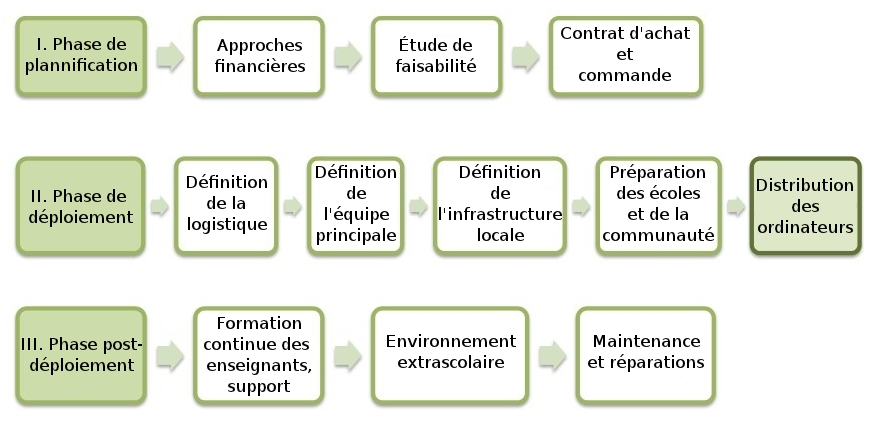
\includegraphics[width=.9\linewidth]{/home/guerry/install/git/OLPC-Deployment--community--guide/images/1_deploy_phases_overview_fr.jpg}
\caption{Survol des phases de déploiement}
\end{figure}
\section{Mise en oeuvre du projet}
\label{sec-4}


Un projet OLPC a un impact évident sur les enfants et leur éducation mais
également sur le système scolaire (en particulier les enseignants), les
familles des enfants ainsi que sur la communauté dans son ensemble : il est
donc important d'en tenir compte lors de la définition des objectifs et
stratégies à mettre en oeuvre. Pour que le projet soit viable, ces
stratégies doivent inclure différents volets ; ceux-ci, ainsi que leur
structuration, sont indiqués dans la pyramide ci-dessous.

L'infrastructure est la base de la pyramide : c'est elle qui fournit
l'accès aux XO, au réseau électrique (ou à une source d'énergie
alternative), à Internet et aux serveurs de l'école ; sans elle, remonter
la pyramide est particulièrement ardu et amène peu de résultats
positifs. Le tiers supérieur de la pyramide propose pour sa part deux types
d'évaluations :

\begin{figure}[htb]
\centering
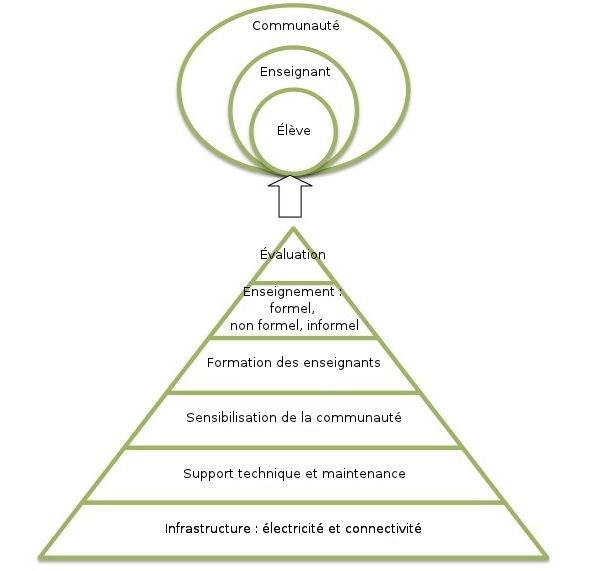
\includegraphics[width=.9\linewidth]{/home/guerry/install/git/OLPC-Deployment--community--guide/images/2_project_implementation_fr.jpg}
\caption{Pyramide résumant l'implémentation d'un déploiement}
\end{figure}

Le premier type permet de mesurer l'impact du projet, sur l'apprentissage
des élèves par exemple, ses effets au niveau social et au niveau des
avancées éducatives. Le second type identifie les secteurs qui sont à même
d'améliorer sa mise en oeuvre. Tous ces éléments se situent dans un cycle
permanent où la partie supérieure de la pyramide donne sans cesse un retour
sur les autres parties.
\subsection{L'équipe principale}
\label{sec-4-1}


\index{Equipe principale!Survol}

Pour une mise en oeuvre réussie, nous recommandons vivement de mettre en
place une équipe locale qui aura des compétences en gestion, logistique,
technique et éducation ; cette équipe se nommera « équipe principale » et
sera l'interface entre le projet et OLPC.

Il est important d'engager un responsable d'équipe possédant de
l'expérience en planification de projet et de budget, en relations externes
et en communication ; il doit être à même de planifier et de coordonner
toutes les opérations ainsi que de superviser les différents secteurs
impliqués ; il doit également posséder une formation dans le domaine
technique ou éducatif. Ce sera à lui de sélectionner les membres de son
équipe selon l'organigramme suivante :

\begin{figure}[htb]
\centering
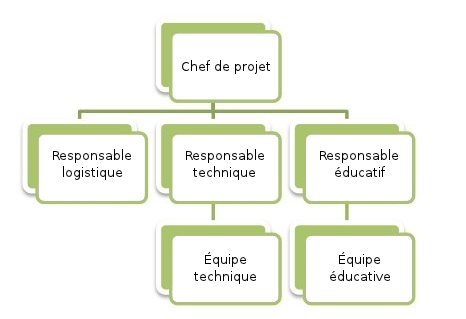
\includegraphics[width=.9\linewidth]{/home/guerry/install/git/OLPC-Deployment--community--guide/images/3_core_team_fr.jpg}
\caption{Structure de l'équipe principale}
\end{figure}

Pour de grands déploiements (>50.000 unités), la totalité de l'organigramme
est indispensable ; le chef de projet devra engager des responsables
éducatif et technique afin de coordonner les actions liées à leur domaine
d'expertise ainsi qu'un responsable logistique qui sera en charge du
stockage des XO, de leur inventaire et de la gestion des pièces de
rechange.

Pour de plus petits déploiements (<2.500 unités), le chef de projet ou le
directeur technique pourra se charger lui-même de la logistique.

Ce tableau donne des informations complémentaires sur les responsabilités
et compétences des membres de l'équipe principale :

\index{Equipe principale!Compétences}
\index{Equipe principale!Diagramme}

\begin{longtable}{|p{2cm}|p{5cm}|p{8cm}|}
\caption{Responsabilités et compétences de l'équipe principale} \\
\hline
 Equipe                     &  Domaines de compétences                                      &  Responsabilités                                                                                                                \\
\hline
\endhead
\hline\multicolumn{3}{r}{Continued on next page}\
\endfoot
\endlastfoot
\hline
 Direction du projet        &  Planification de projet                                      &  Etablissement des règles du projet                                                                                              \\
                            &  Budget                                                       &  Création, supervision et support des équipes techniques et éducatives locales                                                   \\
                            &  Relations externes                                           &  Informations à la communauté et relations publiques                                                                             \\
                            &  Communication                                                &  Distribution des XO                                                                                                             \\
                            &                                                               &  Vérification de l’avancement du projet                                                                                          \\
                            &                                                               &  Rapports d’évaluation                                                                                                           \\
                            &                                                               &  Construction des relations et accords avec les chefs de la/des communauté/s et/ou les institutions gouvernementales             \\
\hline
 Logistique                 &  Douanes                                                      &  Stockage des XO et gestion de l’inventaire                                                                                      \\
                            &  Gestion de l’inventaire                                      &  Gestion des pièces de rechange                                                                                                  \\
\hline
 Technique                  &  Linux, logiciels libres                                      &  Logiciels                                                                                                                       \\
                            &  Maintenance et réparation des XO                             &  Matériel                                                                                                                        \\
                            &  Maintenance du LAN                                           &  Connectivité                                                                                                                    \\
                            &  Ingénieurs Telco pour les serveurs                           &  Collaboration avec les prestataires de services locaux pour obtenir l’énergie appropriée ou l'infrastructure  réseau sur place  \\
                            &  d’école et les systèmes d’inventaires                        &  Maintenance et réparation des XO et serveurs d'école                                                                            \\
                            &  Administrateurs de systèmes                                  &  Gestion du système de sécurité                                                                                                  \\
                            &  Localisation des logiciels                                   &  Construction de capacités techniques adaptées à l’environnement scolaire                                                        \\
\hline
 Education / apprentissage  &  Enseignement                                                 &  Formation et suivi des enseignants                                                                                              \\
                            &  Planning de cours et de développement                        &  Développement du contenu éducatif                                                                                               \\
                            &  Capacité à collaborer avec les enseignants et les étudiants  &  Développement du matériel pédagogique pour les enseignants et les écoles                                                        \\
                            &  Aptitude à diriger                                           &  Développement des programmes éducatifs en cours                                                                                 \\
\hline
\end{longtable}
\section{Stratégie de support}
\label{sec-5}


\index{Assistance}
\index{Support!Strategie}

OLPC apporte un soutien durant les étapes du déploiement, tout
particulièrement dans les domaines opérationnel, éducatif et technique (qui
sont les plus importants).

Pour que la maîtrise du déploiement soit locale et que celui-ci soit
autonome, nous aidons à créer et stimuler des compétences dans les domaines
technique et éducatif, en apportant à l'équipe principale la formation
nécessaire durant le pré-déploiement, puis une assistance à distance
(courriel, téléphone ou chat) durant le postdéploiement, et ceci selon les
besoins du projet.

Ce support est gratuit (quelle que soit la taille du projet). Pour ceux de
25.000 unités et plus, une équipe OLPC éducative et technique se rend dans
le pays du déploiement et y assure une formation complète d'une
semaine. Ceci est aussi valable pour de plus petits projets (5.000 unités
et +) montrant un fort potentiel de croissance à court terme. Pour ceux de
plus de 50.000 unités, la formation initiale peut être étendue à deux
semaines et comporter deux sessions supplémentaires d'une semaine chacune
sur une période d'un an.

Des visites ponctuelles pour un suivi sur place peuvent être faites sur
demande ; une formation éducative complémentaire à la formation initiale
peut être apportée 2-3 fois par an. Nous prenons en charge ces coûts de
formation sur place (à l'exception du matériel et des fournitures), même si
en général, les sponsors fournissent un logement approprié à l'équipe OLPC.
Dans des environnements très difficiles, nous pouvons envoyer une équipe à
plein temps comprenant le chef de projet et les directeurs technique et
éducatif. Le coût de ce type de service OLPC est à négocier lors de la
demande.
\subsection{Support opérationnel}
\label{sec-5-1}


Durant la phase de planification du déploiement et lorsque des décisions
stratégiques sont à prendre (concernant le financement, les contrats et le
processus de commande), nous apportons un support direct au chef de projet
et aux sponsors ainsi qu'un support logistique à la chaîne
d'approvisionnement.
\subsection{Support éducatif}
\label{sec-5-2}


\index{Dévelopement!Educatif}

Lorsqu'un projet est officiellement implanté, nous proposons des ateliers
aux équipes principales afin qu'elles soient à même de mieux appréhender le
XO comme outil d'apprentissage. Durant la phase de structuration, nous
apportons des conseils aux écoles ou centres d'enseignement. Finalement, un
support continu sur le déploiement et le contenu éducatif est amené à
travers les différentes phases de formation aux enseignants par OLPC.
\subsection{Support technique}
\label{sec-5-3}


\index{Support!Technique}
\index{Dévelopement!Technique}

Nous nous concentrons aussi sur la création et la stimulation des capacités
locales telles que la mise en oeuvre de l'infrastructure, la connectivité et
tout autre impératif concernant les logiciels, le matériel, la maintenance
et la réparation des XO.
\subsection{Support par des volontaires et des stagiaires}
\label{sec-5-4}


\index{Volontaires}
\index{Stagiaires}

Durant les mois de juin, juillet et août, nous proposons des stages aux
étudiants de grandes universités de plusieurs pays, le but étant de leur
permettre de travailler main dans la main avec l'équipe principale selon
leur formation et leur domaine d'étude.
\section{Phase de planification}
\label{sec-6}


La phase de planification débute avec l'idée de commencer un projet avec
OLPC et se termine une fois que la commande est passée avec le
constructeur. OLPC aide les responsables du projet à prendre certaines
décisions durant cette phase, ainsi qu'à définir les actions requises en
accord avec les objectifs du programme. Durant cette phase, l'équipe peut
bénéficier d'une meilleure compréhension des divers éléments en rapport
avec un déploiement, que ce soit sur des aspects humains, techniques ou
financiers. Les éléments inclus dans la phase de phase planification sont :
l'étude de différentes approches de financement, l'étude de faisabilité
ainsi qu'un contrat d'achat suivi par une commande de XO.

\begin{figure}[htb]
\centering

\includegraphics[width=.9\linewidth]{/home/guerry/install/git/OLPC-Deployment--community--guide/images/7_planning_phases_fr.jpg}
\caption{De la phase de planification à la commande}
\end{figure}
\subsection{Approches financières}
\label{sec-6-1}


Dans l'idée d'un déploiement OLPC, l'équipe chargée du projet choisit
généralement l'une des trois approches suivantes :
\subsubsection{Ciblage géographique}
\label{sec-6-1-1}


Par l'approche géographique, l'équipe de déploiement sélectionne une région
qui l'intéresse particulièrement. Il peut s'agir d'un pays, d'un état,
d'une ville ou d'une communauté. Une approche par plusieurs villes n'est
pas recommandée car il en découle une utilisation moins efficace de
l'infrastructure et de l'administration, ce qui réduit le nombre d'enfants
touchés. Lorsque le choix se porte sur une région, l'équipe doit pouvoir en
déterminer le nombre d'élèves, d'enseignants et d'écoles. Il faut également
déterminer le nombre d'écoles ayant de l'électricité et celles possédant
une connexion Internet. Avec ces cinq informations, l'équipe peut utiliser
l'étude de faisabilité disponible en annexe afin de déterminer le budget
annuel pour le projet et décider ainsi si une approche progressive est
nécessaire compte tenu des contraintes budgétaires.
\subsubsection{Contraintes budgétaires}
\label{sec-6-1-2}


De nombreuses équipes de déploiement contactent OLPC avec un pays
sélectionné et un budget fixé pour soutenir le projet. En travaillant avec
OLPC, 2 à 4 heures sont nécessaires afin que l'équipe puisse déterminer le
nombre d'élève pouvant bénéficier du projet. Afin que le procédé soit
efficace, les informations suivantes sont requises :

\begin{itemize}
\item Le nombre moyen d'élèves par école.
\item Le nombre moyen d'enseignants par école.
\item Le pourcentage d'écoles ayant l'électricité.
\item Le pourcentage d'écoles connectées à Internet.
\end{itemize}
\subsubsection{Objectifs politiques et sociaux}
\label{sec-6-1-3}


Certaines équipes de déploiement voient un moyen d'obtenir un changement
politique ou social au travers d'un projet OLPC. Par exemple, le
gouvernement d'Uruguay a entrepris le projet CEIBAL afin de favoriser
l'insertion sociale. Cette approche ne présente pas un défi pour OLPC, en
fait cela conduit bien souvent à l'élaboration d'une stratégie de conduite
de projet bien plus rapidement que lors des deux autres approches. Par
l'utilisation du modèle de faisabilité et des quatre informations mises en
avant dans l'approche budgétaire, n'importe quel projet politique ou social
peut-être traduit en budget et en nombre d'ordinateurs à déployer.
\subsection{Principes clés}
\label{sec-6-2}


Il est important pour l'équipe chargée du déploiement de comprendre
certains point clés concernant les coûts impliqués dans la réalisation du
projet :

\begin{itemize}
\item Nous recommandons que l'équipe dispose de personnes à temps plein et sans
  autres responsabilités pour gérer le déploiement,. Idéalement, une
  nouvelle société, association ou agence gouvernementale doit être formée
  pour assumer cette responsabilité. Bien qu'une telle approche puisse
  paraître plus coûteuse, OLPC estime que ce coût est plus que compensé par
  une gestion du projet plus efficace. Cette séparation est également saine
  quant à la gestion au jour le jour et à la politique lors de déploiement
  soutenus par un gouvernement.
\item Le personnel pédagogique est la clé d'un déploiement réussi, tant au
  départ que par la suite. Par conséquent, le budget prévoit que chaque
  écoles soit visitée au moins une fois un mois après la formation initiale
  afin de renforcer la formation et les compétences des enseignants. Des
  dépenses importantes sont également prévues pour la connectivité et la
  gestion du réseau de l'école, mais aussi pour la maintenance des portails
  destinés aux enseignants, élèves, parents et à la communauté.
\item Nous recommandons de disposer d'un centre d'appel pour le projet, afin de
  pouvoir fournir un service de support ou une aide technique aux élèves,
  parents et enseignants. Ce centre s'occupera également de la réparation
  des unités défectueuses. Le budget, basé sur des statistiques historiques
  et incluses dans le modèle, comprend les pièces de rechange. Le besoin en
  réparation varie en fonction de l'utilisation de l'ordinateur par
  l'enfant.
\item Le coût de l'électricité et de la connectivité dépend fortement du pays
  ciblé et de la disponibilité du service. Le modèle comprend tous les cas
  de figure : d'un environnement sans électricité ni connexion à un
  environnement disposant de services complets tels que ceux disponibles
  aux États-Unis. Mener une enquête détaillée par des professionnels dans
  chaque école améliore fortement la justesse du modèle. Le facteur le plus
  susceptible d'être négligé est l'augmentation de la consommation
  d'électricité dans les écoles lorsque les enfants reçoivent puis
  utilisent leurs ordinateurs.
\item Un surcoût important peut s'ajouter avec les droits d'importation et les
  taxes. OLPC n'offre pas de conseils juridiques ou fiscaux et ne participe
  pas aux programmes visant à réduire ou éviter les impôts et les taxes. La
  détermination du montant de telles dépenses est de l'ordre des
  responsables du déploiement. Cependant, OLPC fournit une estimation des
  coûts pour le fret et l'assurance et définit le prix d'un ordinateur en y
  incluant le coût, l'assurance et le transport. Étant donné qu'OLPC a une
  plus grande expérience en organisation de fret maritime, en provenance de
  la Chine avec DHL, que la plupart des équipes chargées d'un déploiement,
  il est recommandé que le chargé du déploiement permette à OLPC de s'en
  occuper. OLPC ne définit pas le prix du fret ni de l'assurance.
\end{itemize}
\subsection{Hypothèses financières}
\label{sec-6-3}


\index{Finance!Hypothèses}

Le tableau suivant propose une répartition des coûts associés à l'exécution
d'un projet. Le premier groupe d'hypothèses se réfère à des coûts non
récurrents, tels que le matériel, l'expédition et l'installation électrique
(si nécessaire). Le second groupe prend en compte les coûts récurrents tels
que les coût d'exploitation mensuels et le salaire des employés.

\begin{longtable}{|l|l|}
\caption{Estimation des coûts d'un déploiement OLPC} \\
\hline
 Estimation des coûts d’installation               &  Estimation des coûts mensuels                     \\
\hline
\endhead
\hline\multicolumn{2}{r}{Continued on next page}\
\endfoot
\endlastfoot
\hline
 \textbf{Coûts généraux :}                         &                                                     \\
 Coût par unité :                                  &                                                     \\
 - Coût FOB                                        &                                                     \\
 - Fret                                            &                                                     \\
 - Droits de douane et taxes                       &                                                     \\
 - Total                                           &                                                     \\
 Coût total des unités déployées                   &                                                     \\
 Contingences 0\%                                  &                                                     \\
\hline
 \textbf{Coûts administratifs et opérationnels :}  &  \textbf{Coûts administratifs et opérationnels  :}  \\
 Location                                          &  Location                                           \\
 Fournitures                                       &  Fournitures                                        \\
 XO                                                &  XO                                                 \\
 Support de bureau                                 &  Support de bureau                                  \\
 Fournitures de bureau                             &  Fournitures de bureau                              \\
 Electricité                                       &  Electricité                                        \\
 Maintenance                                       &  Maintenance                                        \\
 Communications téléphoniques                      &  Communications téléphoniques                       \\
 Transport                                         &  Transport                                          \\
 Voyages et déplacements                           &  Voyages et déplacements                            \\
 Transactions financières                          &  Transactions financières                           \\
 Evaluation                                        &  Evaluation                                         \\
 Juridique                                         &  Juridique                                          \\
 TOTAL                                             &  TOTAL                                              \\
\hline
                                                   &  \textbf{Salaires (par employé)}                    \\
                                                   &  Niveau décisionnel                                 \\
                                                   &  Niveau direction                                   \\
                                                   &  Personnel qualifié                                 \\
                                                   &  IT                                                 \\
                                                   &  Pédagogique                                        \\
                                                   &  Employés non-qualifiés                             \\
\hline
 \textbf{Coûts en électricité}                     &  \textbf{Coûts en électricité}                      \\
 Installation du réseau                            &  Puissance du réseau par kWh                        \\
 Générateur au diesel/gasoline                     &  Coût en carburant par litre                        \\
\hline
 \textbf{Coûts de connectivité}                    &  \textbf{Coûts de connectivité}                     \\
 Modem Dsl                                         &  Coût mensuel du modem Dsl                          \\
 Terminal Satellite                                &  Coût mensuel du terminal satellite                 \\
 Modem GSM                                         &  Coût mensuel du modem GSM                          \\
\hline
\end{longtable}
\section{Étude de faisabilité}
\label{sec-7}


L'étude de faisabilité peut fournir des données pour les besoins des prises
de décision et de budget. Nous recommandons aux sponsors du projet de
concrétiser cette étude afin qu'ils se donnent une meilleure compréhension
des spécificités de la population visée et de l'infrastructure
locale. Après l'ébauche des contours des approches de financement et des
objectifs du programme, d'autres éléments méritent d'être analysés avant de
poursuivre. Le processus de sélection mené par l'école (ou le centre
éducatif) devrait s'appuyer sur les objectifs du programme tels que la
saturation basée sur les niveaux d'apprentissage, la saturation basée sur
la région ou la circonscription ou encore celle basée sur des programmes
spécialisés. Impliquer les écoles au départ permet  d'encourager les chefs
d'établissement à apporter une réponse positive au programme et de
faciliter l'appropriation du projet au niveau de l'école. Une étude de
faisabilité devrait donc prendre en compte :

\begin{itemize}
\item une enquête au sein de l'école ;
\item l'état de l'alimentation et de la connectivité ;
\item l'affectation des ordinateurs portables (stockage et processus de
  distribution) ;
\item les ressources humaines (implémentation du programme).
\end{itemize}

Une fois la sélection des écoles réalisée, une enquête au niveau scolaire
devrait recueillir des informations telles que le nombre de salles de
classe, d'étudiants, d'enseignants et d'administrateurs. Il est important
de garder présent à l'esprit la question de l'accessibilité des écoles au
moment de la planification de la distribution des ordinateurs portables et
des pièces de rechange, ainsi qu'au moment de la conception des structures
dédiées à l'assistance et à la supervision du programme . Par ailleurs,
dans le cadre de l'étude de faisabilité, il convient de réaliser une
évaluation de l'alimentation électrique, de l'infrastructure et de la
connectivité dans chaque école. Les résultats de l'évaluation serviront à
réviser les plans de calendrier et de coûts et afin d'atténuer les écarts
en matière de maturité des écoles. L'évaluation devrait intégrer la
disponibilité du réseau d'alimentation en énergie (ou de sources
alternatives telles que les générateurs ou les panneaux solaires) et la
capacité électrique (en watts), la disponibilité de prises dans chaque
salle de classe, le nombre de serveurs d'école requis ainsi que la
disponibilité d'Internet (DSL, VSAT ou GSM).

L'équation ci-après peut être utilisée afin d'estimer les exigences en
matière d'alimentation électrique pour chaque école. (Les watts-heure sont
fonction de la durée de présence des enfants à l'intérieur de l'école, du
fait qu'ils chargent ou non leurs batteries tout en travaillant, et du
nombre d'heures pendant lesquelles la connectivité est assurée
quotidiennement.)

\begin{figure}[htb]
\centering
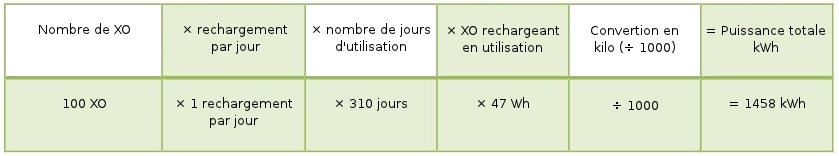
\includegraphics[width=.9\linewidth]{/home/guerry/install/git/OLPC-Deployment--community--guide/images/9_feasibility_study_fr.jpg}
\caption{Besoins en alimentation électrique}
\end{figure}

L'énergie totale requise afin de faire fonctionner 100 ordinateurs
portables et un serveur d'école sur une période de huit heures représente
près de 570 watts multipliés par 8 heures, soit 4560 watts-heure. Ainsi, si
cette énergie devait être générée et stockée sur une période de 2 heures,
il serait nécessaire de disposer d'une capacité de génération approximative
de 11 400 watts pour alimenter un système de batteries doté d'une capacité
de stockage adéquate, en supposant une efficacité de 80\%.
\subsection{Panneaux solaires}
\label{sec-7-1}


Si le déploiement se situe dans un lieu distant et isolé n'ayant pas accès
à l'électricité, les panneaux solaires peuvent être une solution
alternative, pour autant que les panneaux solaires fonctionnent sur 10 et
15 watts. Le panneau de 10 W en sortie à 100 \% pourra recharger une
batterie en moins de trois heures si le XO est éteint. S'il est allumé, le
panneau solaire de 10 W exposé en plein soleil fournira suffisamment de
puissance moyenne pour faire marcher le XO et charger lentement la batterie
(en près de six heures).
\section{Contrats d'achat et processus de commande}
\label{sec-8}


Ce chapitre décrit le processus habituel précédant la commande des
ordinateurs portables ; il indique les décisions à prendre en ce qui
concerne les aspects techniques des XO et les accords contractuels en
découlant.
\subsection{Choix du XO}
\label{sec-8-1}


\index{XO}

Le XO pouvant être fabriqué de différentes manières, il s'agit de choisir
ce qui conviendra le mieux au contexte local du déploiement.
\subsubsection{Claviers}
\label{sec-8-1-1}


\index{XO!Clavier}

Les claviers des XO peuvent être fabriqués pour différentes langues. Afin
que le clavier soit disponible, une image haute-résolution de la
disposition doit être disponible et le logiciel existant doit pouvoir
prendre en charge cet agencement de clavier. Les logiciels d'OLPC sont
conçus pour s'adapter à différents claviers.
\subsubsection{Adaptateurs secteur}
\label{sec-8-1-2}


\index{XO!Adaptateurs secteurs}

Il existe deux types d'adaptateurs, l'un pour des prises murales et l'autre
en bloc d'alimentation. L'adaptateur AC pour le XO dispose d'une entrée
100-240 volts ; trois options sont disponibles :

\begin{itemize}
\item 2 broches plates (US)
\item 2 broches rondes (EU)
\item 3 broches plates (UK)
\end{itemize}
\subsubsection{Mémoire}
\label{sec-8-1-3}


\index{XO!Mémoire}

Le XO utilise de la mémoire SSD (mémoires à semi-conducteurs, de l'anglais
« solid state memory ») en lieu et place d'un disque dur. Ceci est
principalement fait pour augmenter sa solidité mais aussi pour améliorer
ses performances et réduire sa consommation d'énergie. Le type de mémoire
par défaut est d'1 Gio de RAM et de 4 Gio de mémoire flash. En fonction du
budget et des conditions d'utilisation, il est possible de sélectionner un
SSD plus rapide ou plus important afin que le XO puisse améliorer ses
performances et sa capacité de stockage.
\subsection{Contrat d'achat}
\label{sec-8-2}


OLPC s'engage à reconnaître le soutien d'un sponsor à un projet une fois
qu'elle a reçu un contrat signé ainsi qu'une lettre de crédit en sa faveur
à raison de 100\% de la valeur des XO. OLPC accepte également des
transferts de paiement par télex en lieu et place de lettres de crédit.

Le contrat d'achat comporte cinq sections importantes :

\begin{enumerate}
\item les spécifications détaillées du XO, comprenant la configuration mémoire
   RAM et flash ;
\item le nombre d'ordinateurs commandés ainsi que le prix CIF de chaque
   ordinateur ;
\item la date de livraison ;
\item les termes de guarantie et de conditions d'utilisation ;
\item les chapitres légaux standards, tels que les lois gouvernementales et
   résolution de problèmes.
\end{enumerate}


Lors de l'achat d'une grande quantité de XO, OLPC travaille selon un accord
contractuel précisant les modalités et conditions des commandes de XO. OLPC
a un modèle de contrat qui peut être modifié en conformité avec les
exigences du déploiement. Les points abordés dans le contrat OLPC incluent
les termes de paiement, la garantie, les directives concernant la lettre de
crédit ainsi que d'autres points concernant le processus
d'approvisionnement en XO.  Le personnel financier d'OLPC travaille en
étroite collaboration avec la chaîne d'approvisionnement et la logistique
afin de respecter et garantir les délais et conditions énoncés dans
l'entente contractuelle.
\subsubsection{Modalités de paiement et Incoterms}
\label{sec-8-2-1}


\index{XO!Paiement}
\index{Incoterms}

L'option de paiement la plus courante pour les commandes de XO à grande
échelle est de 20 \% par acompte et de 80 \% payable par lettre de crédit
transférable. Le modèle OLPC permettant d'établir des lettres de crédit
transférables peut être trouvé dans le contrat d'OLPC. Le personnel
financier d'OLPC s'engage à répondre efficacement et rapidement aux
questions financières relatives à l'achat. L'Incoterm utilisé pour l'achat
de grandes commandes de XO est le CIF (coût, assurance et fret, Incoterms
2010). Le terme CIF signifie que le vendeur (OLPC) est responsable des
coûts d'expédition et d'assurance du pays d'origine au port de
destination.

L'acheteur de la cargaison est responsable de tous les coûts associés au
transport une fois que les marchandises sont livrées au port de
destination. Ces coûts comprennent l'entrée des douanes et le prix de
dédouanement, les droits et taxes d'entrée, les surtaxes, les redevances
d'amerrissage au port de l'importateur, le déchargement sur des camions à
ce port et la livraison à la destination finale.
\subsubsection{Garantie}
\label{sec-8-2-2}


\index{Garantie}

Toutes les commandes de XO sont livrées avec 1 \% d'unités supplémentaires
en lieu et place d'une garantie conventionnelle sur le matériel. Ces unités
sont expédiées sans frais supplémentaires. De plus, OLPC fournit une
garantie limitée en cas de problème sur la série. Les détails sur cette
garantie sont dans le contrat d'OLPC.
\subsubsection{Frais de douane et taxes}
\label{sec-8-2-3}


\index{Douane}

Les frais de douanes et taxes associés au transport des XO varient selon
les règles en vigueur des douanes locales. Les frais de douane sont parfois
très élevés, allant jusqu'à atteindre 20\% de la valeur commerciale. Afin
d'éviter de telles taxes, OLPC recommande à l'équipe locale d'effectuer des
recherches afin d'obtenir une exonération fiscale lorsque cela est
possible.

\index{Exonération fiscale}

Obtenir une exonération fiscale sur les XO importés à des fins éducatives
peut demander l'autorisation d'un certain nombre de collectivités locales,
ce qui peut amène à une organisation plus importante. Les autorités
douanières locales doivent être consultées sur ce procédé, ce qui permet
également d'obtenir une idée du temps nécessaire pour l'obtention d'une
reconnaissance d'exemption. OLPC fournit toute la documentation nécessaire
pour une demande d'exemption auprès des autorités locales.
\subsubsection{Pièces de rechange}
\label{sec-8-2-4}


\index{XO!Pièces de rechange}


Des pièces de rechange pour les XO peuvent être achetées en même temps que
la commande initiale de XO et également par la suite. OLPC peut aider
l'équipe en charge pour l'achat de pièces détachées au
constructeur. Celles-ci sont disponibles pour des commandes en quantité
minimale. Si les pièces de rechange sont achetées lors de la commande
initiale, OLPC peut recommander certaines pièces en particulier ainsi que
les quantités requises.

La logistique OLPC, basée à Miami en Floride, suit chaque commande depuis
la réception de la lettre de crédit jusqu'à la livraison de la commande au
port de destination. Il est de la responsabilité des commanditaires locaux
de faire passer la douane aux unités commandées. L'équipe locale est seule
responsable des transports suivants et des taxes, frais et autres coûts qui
y seraient liés ainsi que de tous les frais de transfert des ordinateurs du
quai à l'entrepôt.
\subsection{Processus de commande de XO et délai de production}
\label{sec-8-3}


\index{XO!Commande}
\index{XO!Délai de production}

Afin de minimiser le coût final, OLPC fabrique les XO lors de chaque
commande afin de ne pas à avoir à maintenir un inventaire. Officialiser
l'engagement d'achat de XO permet à OLPC de travailler avec l'équipe
principale pour l'établissement d'un calendrier de déploiement permettant
un déploiement efficace.

Dès réception du paiement (paiement d'avance ou lettre de crédit), OLPC
envoie un ordre d'achat au producteur qui prend 1 à 2 semaines de
traitement. Il faut normalement 12 à 16 semaines pour fabriquer les XO. Le
fabriquant peut produire 240.000 XO par mois pour OLPC, bien que des
commandes préexistante d'OLPC risquent de réduire cette capacité. Cependant
peu de projets peuvent traiter l'arrivée de plus de 50.000 XO en un seul
mois. OLPC prévoit normalement six semaines pour l'expédition maritime des
XO. La livraison de ceux-ci par avion prend moins de temps mais en raison
du coût de fret aérien, il n'est pas recommandé.

Le temps de transit estimé pour une livraison par fret maritime est de 1 à
6 semaines une fois que les XO sont disponibles chez le fabricant. Lors de
la planification du déploiement, veuillez prévoir de 14 à 24 semaines entre
le reçu du paiement et la date à laquelle vous pouvez estimer recevoir les
XO dans le port désigné. OLPC travaillera avec votre équipe de déploiement
afin d'établir un calendrier de livraison. Selon la quantité de XO
commandés, la livraison sera effectuée en une ou plusieurs fois. Les
questions à prendre en compte lors de l'élaboration de votre calendrier de
livraison des XO devraient comprendre : la date à laquelle les XO sont
nécessaires pour la formation des enseignants, le temps requis pour faire
l'inventaire des livraisons, le temps de transit de la livraison finale des
XO à leur destination ou sur un site de distribution, etc. Ces informations
aideront OLPC, via l'équipe principale, à établir un calendrier de
livraison des XO complet et efficace.

\begin{figure}[htb]
\centering
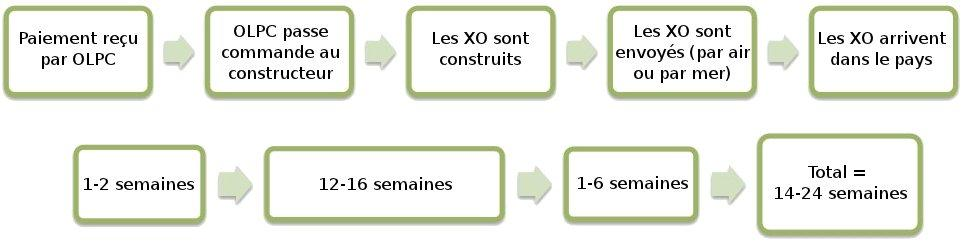
\includegraphics[width=.9\linewidth]{/home/guerry/install/git/OLPC-Deployment--community--guide/images/10_xo_order_process_fr.jpg}
\caption{Processus de commande des XO}
\end{figure}
\section{Phase de déploiement}
\label{sec-9}


La phase de déploiement comprend tous les événements qui se produisent
entre la commande du XO au fabriquant et sa distribution finale aux écoles
et enfants. Le délai d'exécution alloue du temps pour le recrutement des
membres de l'équipe principale et pour son organisation d’une formation
technique et pédagogique OLPC. En outre, ce temps peut être utilisé pour
satisfaire les besoins en infrastructure sur la base des résultats de
l'étude de faisabilité.

Les espaces de stockage doivent être prêts pour l'arrivée des XO, tout
comme doit l'être le personnel en charge de la gestion des stocks et du
processus de distribution.

Les chefs d'établissements scolaires et les administrateurs doivent être
informés des objectifs et  implications du programme dès les premières
étapes du projet. Des réunions formelles entre ces parties et d'autres
membres compétents du système éducatif ou des personnalités politiques
devraient être organisées pour mettre en place un calendrier sur la
formation des enseignants et des autres activités au niveau de l'école.

Une fois les XO parvenus dans le pays, les étapes à suivre incluent
notamment la mise en place de la logistique, de la formation de l'équipe
principale par OLPC, de la mise en place des infrastructures scolaires
ainsi que la préparation des écoles et des communautés au déploiement des
XO.

\begin{figure}[htb]
\centering
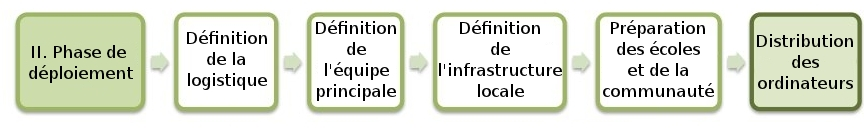
\includegraphics[width=.9\linewidth]{/home/guerry/install/git/OLPC-Deployment--community--guide/images/11_deploy_phases_fr.jpg}
\caption{De la phase de déploiment à la distribution des XO}
\end{figure}
\subsection{Mise en place de la logistique}
\label{sec-9-1}


\index{Logistique}

Le département logistique de l'équipe principale est responsable de la
logistique dès l'arrivée des XO à leur port de destination. Le responsable
de la logistique est en charge du dédouanement et de la livraison jusqu'à
sa destination finale. Un processus logistique efficace et rapide est non
seulement important pour maintenir le calendrier de déploiement proposé,
mais également essentiel pour éviter les frais ou taxes pouvant être
appliqués en cas de retard dans le dédouanement ou le déchargement lors de
son arrivée au port de destination.

Une fois les XO arrivés au port de destination, puis dédouanés et
entreposés dans l’entrepôt de stockage, trois tâches principales doivent
être effectuées :

\begin{enumerate}
\item Les XO doivent être inspectés individuellement concernant d'éventuels
   dommages subis pendant le transport, et les réclamations d'assurance
   éventuelles doivent être prêtes.
\item Les XO peuvent avoir besoin d’être configurés avec la dernière version
   du système d'exploitation et tout son contenu local s'il y a eu des
   modifications apportées au logiciel depuis le moment où les unités ont
   été expédiées. Cette procédure confirme aussi que les XO sont en ordre
   de marche et prêts pour les élèves et les enseignants.
\item Les numéros de série des ordinateurs ainsi que les numéros
   d'identification de chaque élève et enseignant doivent être entrés dans
   le système de gestion de stock. Cette procédure apporte des informations
   basiques qui seront ensuite mises à jour afin de refléter l'historique
   des réparations, les transferts ou les remplacements des XO.
\end{enumerate}
\subsubsection{Entreposage}
\label{sec-9-1-1}


\index{Entreposage}

Lorsque l'on élabore des plans pour le stockage local des XO, il est
important de prendre en compte la sécurité des installations de stockage,
l'impact des conditions météorologiques sur les XO stockés, et la
couverture d'assurance éventuellement requise.

Le département en charge des opérations peut fournir des informations sur
les dimensions d'emballage ou sur toute autre interrogation concernant
l’emballage.

L’entreposage local permet de stocker les XO en vue de leur configuration
tandis que l’infrastructure logistique est prête à acheminer les XO. Un
positionnement stratégique d’entrepôts régionaux permet de réduire le coût
logistique et améliore l'efficacité de la réparation et du remplacement des
XO.
\subsubsection{Plan de distribution des ordinateurs portables}
\label{sec-9-1-2}


\index{Distribution}

Dans l'expérience OLPC, la plupart des sponsors peuvent distribuer au
maximum 60.000 XO par mois. Ils sont généralement distribués par des
sociétés tierces, l'armée, ou des organisations de coopération
multilatérale, comme la FAO ou le PAM. Celles-ci ont une vaste expérience
dans la sécurisation de la logistique. Dans de nombreux pays, un millier de
XO est une cible de choix pour le vol : la sécurité devrait donc être une
préoccupation primordiale dans le choix d'une entreprise de logistique. Il
serait par ailleurs adéquat que l'arrivée des XO dans les écoles et
communautés corresponde à une festivité et, bien sûr, à une connexion
internet valide.

L'expérience OLPC montre que le meilleur plan de distribution est celui qui
débute avec les zones les plus faciles, sauf s'il faut tenir compte de
considérations politiques. Débuter par les zones les plus simples permet
d’identifier et de mettre en place tous les changements de dernière
minute. Le personnel apprend ainsi aussi plus rapidement quand il peut se
concentrer sur des installations plus simples ne nécessitant pas
l'installation d'équipements solaires ou de relais satellites.
\subsubsection{Gestion des pièces détachées}
\label{sec-9-1-3}


\index{Pièces détachées}

Il s'agit d'une partie souvent négligée, mais qui est pourtant la clé d'un
déploiement réussi. Les XO tombent en panne suite à l'utilisation qu'en
font les enfants; selon notre historique, plus une région est pauvre, plus
les réparations sont fréquentes. Sans surprise, car ces élèves manquent
d'expérience avec les appareils électroniques, les soins appropriés et le
maniement des ordinateurs.

Un projet devrait planifier la réception d'un inventaire de pièces de
rechange dans les 6-9 mois suivant la livraison des XO aux enfants. Jusque
là, le 1\% d'unités excédentaires livrées avec chaque commande doit être
suffisant pour gérer les réparations. Le personnel OLPC en charge de la
logistique peut fournir des conseils sur la composition de la commande
initiale de réparation; avec le temps, le projet devrait baser ses
commandes de pièces détachées sur des données réelles.
\subsubsection{Etude de référence}
\label{sec-9-1-4}


Avant de commencer un déploiement, il est conseillé d'avoir les données
nécessaires au scénario de mise en œuvre du projet. Le chef de projet et
l'équipe principale peuvent collaborer avec des experts en évaluation ou
des institutions académiques/de recherche pour concevoir un cadre
d'évaluation capable de mesurer l'impact du projet selon ses objectifs. Le
cadre d’évaluation mérite d'être aligné avec les mesures d'apprentissage
des élèves, ce qui demande une analyse minutieuse des indicateurs et des
outils.

L'information de base peut servir de point de départ utile pour mieux
comprendre la communauté impliquée dans le projet, et peut même conduire à
la formulation des objectifs que les intervenants souhaitent
atteindre. Elle rend également possible la mesure l'impact d'un projet, car
elle permet aux chercheurs d'analyser et de comparer statistiquement les
données de base avec les données recueillies durant les années de mise en
oeuvre d'un projet.

Les objectifs et résultats attendus du programme devraient être les
critères de sélection du type de données de base à collecter. Des données
administratives peuvent mesurer les changements dans la fréquentation
scolaire, les taux de scolarisation et le taux d’abandon. Les mesures de
l'impact social et comportemental peuvent inclure des enquêtes ou
questionnaires relatifs aux attitudes, motivations et opinions des parents,
élèves et membres de la communauté sur le projet lui-même ou sur
l'apprentissage des élèves. Les performances des élèves peuvent être
mesurées par des épreuves standardisées, locales ou nationales, les examens
traditionnels ne parvenant pas à évaluer les nouvelles compétences
développées par les élèves lors d'une introduction technologique dans leur
apprentissage.

Ces nouvelles dimensions d'apprentissage (résolution de problèmes, pensée
critique, gestion de sources multiples d'information, capacité de
réflexion, communication - visuelle, auditive, interactive, etc. -
utilisant des médias variés, compétences en travaux individuels et en
équipe,  capacités d'auto-apprentissage, dimensions plus complexes
comprenant l'agencement [Carlson \& Earls, 2001], efficacité des enfants et
des jeunes à apporter des changements significatifs à l'environnement dans
lequel ils vivent [Kamo, N. et al, 2008] demandent à être évaluées.
\subsection{Mise en place de l'équipe principale}
\label{sec-9-2}


\index{Equipe principale}

Comme expliqué dans les pages précédentes, ce que nous appelons « équipe
principale » est l'équipe locale ; elle a la responsabilité de la mise en
œuvre des différents composants du déploiement. Nous allons nous concentrer
ici sur les équipes technique et pédagogique. Leur travail est crucial pour
la mise en œuvre réussie du déploiement; son personnel doit être
soigneusement recruté et soutenu financièrement de manière pro-active
durant toute la durée du programme. À ce point du déploiement, il est
crucial d'avoir créé une équipe principale adéquate.

La taille de cette équipe dépendra du nombre d'unités déployé. Bien que les
apprentissages des équipes technique et pédagogique ont à se concentrer sur
des composantes différentes, l'idéal reste un réel travail d'équipe se
communiquant plans, défis et  mises à jour sur une base très régulière. Il
est de la responsabilité du chef de projet de faciliter la mise en place de
ce type de relations au sein de l’équipe. Avoir un leader pour chaque
équipe est réellement souhaitable. Ces leaders ou managers ont à maintenir
une communication constante avec les équipes technique et pédagogique
d’OLPC.

OLPC facilitera l'organisation d'un atelier stratégique avec l'équipe
principale pour :

\begin{enumerate}
\item Renforcer les capacités dans la gestion des XO, dans ses activités et
   utilisations comme outil d'apprentissage.
\item Renforcer les capacités à mettre en place l'infrastructure, la
   connectivité et les autres exigences techniques à l'école ou au niveau
   communautaire.
\item Déterminer la structure de soutien (pour les aspects techniques et
   pédagogiques) qui fonctionnera de l'équipe principale jusqu'à l'école ou
   au centre d'apprentissage.
\item Déterminer et appuyer les stratégies de formation initiale et continue,
   et le développement de contenu pour les écoles et les enseignants.
\item Définir des stratégies pour intégrer les membres de la communauté et la
   famille dans le projet.
\end{enumerate}

La durée de l'atelier peut varier de quelques jours à plusieurs
semaines. Cela dépendra des caractéristiques du projet: la taille de
déploiement (quantité d'ordinateurs portables, échelle et plan de
distribution), l'équipe principale (background et taille), l'emplacement du
projet, les objectifs du projet et de l'état des infrastructures. La durée
dépendra aussi des accords conclus pendant la phase de planification entre
OLPC, le chef de projet et des besoins spécifiques du projet. Le contenu et
les activités de ce premier atelier va également s'adapter aux besoins et à
l'expérience des participants. Toutefois, l'approche/méthodologie et
certains contenus sont communs à tous les ateliers pour qu'ils s'articulent
autour des mêmes principes que nous défendons: apprendre en faisant, en
construisant, en collaborant et en réfléchissant.

Nous recommandons fortement aux managers techniques et pédagogiques de
l'équipe principale de commencer à discuter le contenu, la durée et le
calendrier de cet atelier en consacrant du temps à des webinaires avec
OLPC. Cela permettra à OLPC et aux équipes de déploiement de définir les
détails de l'atelier et pour l'équipe principale pour avancer dans les
préparatifs nécessaires avant la formation.
\subsubsection{Description de la formation OLPC}
\label{sec-9-2-1}


\index{Formation OLPC}

Les objectifs de l'atelier d'apprentissage OLPC peuvent inclure:

\begin{itemize}
\item Développer une compréhension de la théorie de l'apprentissage et de la
  pédagogie OLPC
\item Fournir une expérience pratique de la plateforme d'apprentissage Sugar.
\item Permettre à l'équipe principale d'utiliser le XO dans des stratégies
  efficaces d'apprentissage grâce à la construction, l'expression, et la
  collaboration.
\item Intégrer le mode 1:1 au curriculum et à des environnements
  d'apprentissage informels.
\item Evaluer l'apprentissage au sein des environnements informatiques 1:1.
\end{itemize}

Certains contenus techniques de l'atelier peuvent concerner simultanément
les équipes pédagogiques et techniques, tandis que d'autres sujets avancés
devraient être traités séparément avec l'équipe technique.

Les objectifs de l'atelier technique de l'OLPC peuvent être:

\begin{itemize}
\item Résolutions des problèmes logiciels ou matériels
\item Créer et utiliser un port USB Re-Flash Stick
\item Connexion et inscription au serveur d'école
\item Configuration d'un point d'accès.
\item Installation et configuration du serveur d'école
\item Définir une stratégie de support technique
\item Définir une stratégie d'entretien et de réparation à large échelle en
  milieu scolaire
\end{itemize}

L'ordre du jour qui suit est un échantillon des sujets habituellement
couverts lors d'un atelier d'une semaine avec l'équipe principale:

OLPC propose un suivi des ateliers qui peut être effectué plusieurs mois
après le déploiement soit en marche ou une fois que l'équipe principale a
acquis l'expérience de base, les connaissances et les compétences qui
profitent à leur déploiement. Cette option peut être mise en oeuvre pendant
une formation initiale avec OLPC, si les participants démontrent déjà un
niveau avancé de compétences. Une autre option pour le suivi des formations
consiste en des ateliers spécialisés qui mettent l'accent sur un sujet
d'intérêt particulier pour l'équipe principale et qui visent à développer
des compétences complémentaires et spécialisées. Enfin, OLPC propose des
ateliers régionaux pour répondre aux besoins communs à une région
spécifique. Pour cela, OLPC choisit un lieu stratégique qui permettra aux
participants de multiples déploiements d'y assister.

Les éléments suivants sont des exemples d'ateliers avancés pour l'équipe
principale :

\begin{table}[htb]
\caption{Exemples d'ateliers Sugar avancés} 
\begin{center}
\begin{tabular}{|p{3.8cm}|p{11cm}|}
\hline
 Sujet / Activité                                                             &  Description                                                                                                                                                                               \\
\hline
 \textbf{Programmation et débogage} (recherche des erreurs de programmation)  &  Développement de compétences en programmation et en erreurs de programmation afin que les participants puissent eux-mêmes devenir des meneurs dans des projets avancés de développement.  \\
                                                                              &  Ces stages incluent la démonstration de compétences avancées en programmation Etoys et Python.                                                                                            \\
\hline
 \textbf{Robotique}                                                           &  L’utilisation de senseurs d’autres plates-formes robotiques incluant le XO dans des projets de développement.                                                                             \\
\hline
 \textbf{Communauté Sugar}                                                    &  Contributions des participants à la communauté Sugar par la conception de matériel ou d’activités Sugar pour un contenu local ou pour toute la communauté Sugar.                          \\
\hline
 \textbf{Développement du cursus}                                             &  Le développement d’une base innovatrice de cours alignée sur le cursus local.                                                                                                             \\
\hline
\end{tabular}
\end{center}
\end{table}
\subsubsection{Développement de contenu}
\label{sec-9-2-2}


\index{Contenu!Développement}

Une autre stratégie recommandée pour les équipes de base pour le
déploiement est le développement de contenu pour les communautés et les
écoles. Les documents suivants sont des exemples d'un tel contenu: a) Guide
pour les usages multiples des ordinateurs b) des idées pour des projets qui
correspondent à des thèmes spécifiques, qui pourraient être d'intérêt ou
pertinents dans l'environnement des élèves et des enseignants. c) Les plans
de leçon qui montrent comment utiliser les activités de Sugar lors de
l'enseignement de différentes parties du programme national

Nous recommandons la création d'une première bibliothèque ou portfolio de
projets qui aidera les enseignants à intégrer l'ordinateur dans leur
pratique pédagogique tout en les incitant à créer leurs propres projets, en
se concentrant sur l'approche de formation décrite dans la section
précédente. Il se peut que chaque enseignant utilise l'ordinateur dans leur
classe individuelle, ou que les enseignants de différentes régions se
réunissent pour concevoir des projets communs. De toute façon, cette
approche permettra de rendre explicites les concepts que les projets
intègrent et promeuvent, soulignant ce que l'on peut «manipuler» et
comprendre en utilisant le portable, mais qui serait plus difficile, ou
presque, impossible à réaliser avec le stylo et papier.
\subsection{Préparer les écoles et communautés}
\label{sec-9-3}


\index{Ecoles}
\index{Communautés}

Lorsque les ordinateurs portables sont prêts à être distribués, et en
supposant que les infrastructures scolaires sont prêtes, il est temps de
préparer les enseignants et autres membres des communautés pour cette
expérience. La formation des enseignants et de sensibilisation de la
communauté peuvent se produire simultanément, mais peut également se
produire à différents moments. Des variables liées à la localisation, la
taille et la préparation de chaque école ou communauté doivent être
considérés au moment de décider l'ordre dans lequel mettre en oeuvre chaque
événement.
\subsubsection{Formation des enseignants}
\label{sec-9-3-1}


\index{Formation des enseignants}

La formation des enseignants est une composante essentielle d'un projet
OLPC et devrait être un processus continu. Les enseignants devraient être
les premiers membres de la communauté éducative à recevoir des informations
et à s'impliquer dans des initiatives qui ont des effets directs sur leurs
propres pratiques professionnelles. Il est recommandé de commencer la
formation des enseignants et leur fournir des ordinateurs portables XO dès
les premiers stades d'un projet; cette approche garantissant leur niveau de
confiance et d'engagement dans l'initiative.

L'aspect le plus important de la préparation des enseignants est en ce qui
concerne la manière dont les enfants apprennent. Les éducateurs ont reconnu
depuis longtemps que les enfants apprennent mieux quand ils sont actifs ou
quand ils poursuivent leurs propres intérêts, et quand ils évoluent dans
une culture de la connaissance et de l'engagement.

Avec l'accès en mode 1-to-1 à des ordinateurs portables connectés, les
enfants s'engagent activement dans la construction des connaissances et ne
sont pas limités à la réception passive de l'information. Chaque enfant (et
les enseignants eux-mêmes) peuvent poursuivre leur apprentissage dans des
domaines d'intérêt personnel et la pratique en classe ne se limite pas à
une approche prédéterminé et uniforme.

Les enseignants en bénéficient aussi. Non seulement ils arrivent à utiliser
les ordinateurs portables à la maison pour leur propre apprentissage, mais
l'ordinateur portable connecté devient un moteur pour le développement
professionnel personnalisé. Cela permet aux enseignants d'accéder à
l'expertise et à échanger avec les collègues, en posant et répondant à des
questions pratiques. Ils peuvent participer pleinement en tant que
producteurs de connaissances et non pas seulement comme des consommateurs
de matériel produit par d'autres.

L'équipe principale devrait élaborer différentes stratégies pour développer
la capacité de l'enseignant:

\index{Formation!Ateliers}

\begin{enumerate}
\item Des ateliers de formation: où les enseignants apprennent à utiliser
   l'ordinateur, et, dans le même temps, à l'incorporer dans leur pratique
   pédagogique.
\item Les mécanismes de soutien: Bien que le contenu de l'initiative constitue
   un mécanisme de soutien important à la pratique de l'enseignement,
   d'autres mécanismes doivent être mis en oeuvre, y compris l'assistance en
   classe, ce qui peut se faire grâce à des accords avec des universités,
   des lignes téléphoniques d'aide qui peuvent être mis en place avec des
   techniciens développeurs dans le pays, et blogs ou des forums en ligne
   où les enseignants peuvent participer.
\item Des clubs enseignants: des espaces de travail où les enseignants peuvent
   se rencontrer régulièrement pour partager les réussites, les problèmes
   et solutions.
\item Guides et ressources.
\end{enumerate}

Lors des premières formations, les enseignants devraient apprendre les
utilisations de base de l'ordinateur portable et comment l'intégrer dans
leur pratique pédagogique. La formation devrait être guidée par la vision
et l'objectif de l'initiative globale. Nous recommandons que l'approche
appropriée soit celle de «learning by doing» et que le «faire» se concentre
sur le développement de projets concrets au sein de la classe. L'équipe
principale doit adapter le contenu et la durée de la formation initiale sur
la base des compétences des enseignants.

Il est recommandé que l'équipe technique effectue des sessions de formation
avec l'équipe pédagogique pour préparer les enseignants au dépannage
technique de base concernant les logiciels, le matériel et la
connectivité. Au cours de ces premières sessions avec les enseignants,
l'équipe principale peut rapidement identifier les participants qui font
preuve de leadership et qui peuvent être des contacts clés pour soutenir le
projet au niveau de l'école. Selon l'ampleur du projet, l'équipe principale
peut décider de former les enseignants directement ou par le biais
d'enseignants-formateurs qui seront ensuite amenés reproduire les
formations pour d'autres enseignants. Certains projets décident d'effectuer
des formations à grande échelle dans une démarche visant à cibler plusieurs
écoles.

Les écoles peuvent choisir les membres clés de leur personnel à participer
à cette formation, avec l'idée que ces stagiaires deviennent des leaders et
démultiplient la formation dans leur propre école. Une autre approche
consiste à attribuer à chaque membre de l'équipe principale une école
spécifique dans lequel s'effectue la formation du personnel sur place. Peu
importe l'approche qui est choisie, l'équipe principale a besoin de
surveiller constamment les progrès de chaque école et de chaque
enseignant.

L'ordre du jour qui suit est un échantillon de sujets que l'équipe
principale peut couvrir durant une session de formation initiale des
enseignants :

\begin{table}[htb]
\caption{Une semaine de formation initiale des enseignants} 
\begin{center}
\begin{tabular}{|l|l|}
\hline
 Jour  &  Sujet / activité                                                                    \\
\hline
    1  &  Bienvenue et introduction                                                           \\
       &  Vue d’ensemble OLPC : principe, mission et philosophie                              \\
       &  Modèle pédagogique d’OLPC : le constructionnisme                                    \\
       &  Lectures et réflexions : les enfants, l’apprentissage et les ordinateurs            \\
       &  Travaux pratiques : vue d’ensemble des outils disponibles sur les XO                \\
       &  Introduction au XO : Matériel et logiciels                                          \\
\hline
       &  Introduction aux activités Sugar Logo et Turtle art                                 \\
    2  &  Créer et utiliser un stick Reflash                                                  \\
       &  Résolution de problèmes simples de matériel                                         \\
       &  Utilisation du XO comme outil d’apprentissage                                       \\
\hline
    3  &  Programmation d’activités sur le XO : Scratch                                       \\
       &  Réseaux de collaboration et d’apprentissage                                         \\
       &  Résolutions de problèmes simples de logiciels                                       \\
\hline
       &  Mise en oeuvre du projet : Construire les équipes nécessaires à un bon déploiement  \\
    4  &  Préparation des écoles et des communautés                                           \\
       &  Développement de la capacité locale : formation des enseignants                     \\
       &  Cursus, contenu et matériaux dans un environnement 1-1                              \\
       &  Expérimentation de projets d’apprentissage : élaborer des projets via les XO        \\
\hline
    5  &  Présentation de projets                                                             \\
       &  Intégration des familles et autres membres de la (des) communauté(s)                \\
       &  Energie et connectivité                                                             \\
       &  Evaluation et métriques                                                             \\
       &  Questions et réponses                                                               \\
\hline
\end{tabular}
\end{center}
\end{table}


Le déploiement des ordinateurs portables pour chaque enfant dans toute une
région ou un pays ne peut pas être géré par l'équipe principale seule. Il
doit être mené par l'équipe principale, et soutenu par des équipes
régionales. L'équipe principale devra fixer les principes directeurs du
programme tandis que les équipes régionales seront chargées du déploiement
dans leurs régions respectives en fonction de ces principes, tout en
soulevant des inquiétudes et en proposant des alternatives viables si
nécessaire. Différentes fonctions devraient être déléguées aux équipes
régionales selon les pratiques existantes.
\subsubsection{Sensibilisation des communautés}
\label{sec-9-3-2}


\index{Communauté!Sensibilisation}

Avant l'arrivée des ordinateurs portables dans une communauté, il est
important de préparer les différents groupes de personnes qui seront
touchées par le projet: parents, enseignants, directeurs d'école, les
familles, et d'autres membres actifs d'une communauté. Le ministre de
l'Education, les autorités et leaders et locaux devraient être impliquées
dans les communications au sujet du programme, de ses objectifs, des
caractéristiques, avantages et engagements à prendre.

Les coordonnateurs du projet doit planifier soigneusement les campagnes de
sensibilisation, en sélectionnant les outils appropriés (impressions,
affiches, panneaux, etc) et des stratégies de communication (spots radio ou
de télévision, rencontres, etc) adaptées aux caractéristiques uniques de
chaque communauté et à l'échelle de chaque projet. Le calendrier de la
campagne devrait également être mûrement réfléchi afin de permettre aux
communautés de se préparer à lancer un programme formel. Si des campagnes
nationales sont créées pour informer les différents publics sur les
projets, elles devraient être mises en place avant la distribution des
unités ou après que des actions de sensibilisation communautaire plus
formelles soient entreprises par l'équipe principale.

La phase de préparation joue un rôle important dans la création des
attentes positives, les attitudes, et l'implication de tous les
membres. Lorsque les communautés comprennent les programmes et leurs
avantages, il ya des impacts directs sur l'apprentissage et sur la façon
dont les ordinateurs portables sont pris en charge. Au niveau national et
local, les collectivités doivent savoir ce que signifie un ordinateur
portable par enfant. Les enfants sont les meilleurs ambassadeurs, mais
l'implication des parents et chefs des communautés est également
influente. Encourager la sensibilisation est très important pour le succès
des initiatives, à la fois parce qu'il permet aux familles et autres
membres des communautés d'être impliqués dans le processus d'apprentissage
des enfants, et parce qu'il leur permet d'être des participants actifs dans
la création d'une nouvelle culture et de nouvelles expériences
d'apprentissage au sein de leur communauté.

Les réunions de parents peuvent être tenus dans des écoles ou des centres
communautaires et devrait inclure, sans s'y limiter, les sujets suivants:

\begin{itemize}
\item Une description des responsabilités et des rôles dans les différentes
  phases du projet. Tâches à définir, organisées et réalisées par des
  groupes d'action différents.
\item Établissement de normes pour le partage des ordinateurs portables parmi
  les frères et soeurs et aux enfants plus âgés.
\item Sécurité des ordinateurs portables. Comment et pourquoi prendre soin des
  machines ?
\item Processus de recharge.
\item Accès Internet.
\item Signature de l'accord par les parents.
\end{itemize}

D'autres acteurs peuvent être invités aux réunions afin qu'ils puissent
faire partie de l'initiative et pour matérialiser les accords avec
différents consultants et / ou des bénévoles du projet.
\subsection{Mise en place de l'infrastructure locale}
\label{sec-9-4}


\index{Infrastructure}

Avant l'arrivée des ordinateurs portables, les techniciens de l'équipe
principale devrait évaluer, configurer, tester, et être responsable du
réseau et des infrastructures d'alimentation dans les écoles et / ou
d'autres centres communautaires.

OLPC peut commencer à soutenir l'équipe principale avant la formation dans
le pays grâce à des webinaires en ligne ou les chats. Au cours de la visite
d'OLPC dans le pays la formation pratique a lieu, et l'équipe principale
devrait être prête pour la mise en place de l'infrastructure locale. OLPC
continuera à soutenir les équipes techniques en ligne après l'organisation
de la formation dans le pays.
\subsubsection{Electricité}
\label{sec-9-4-1}


\index{Electricité!Déploiement}

L'infrastructure électrique de l'école doit être évaluée en fonction de la
demande d'électricité générée par des ordinateurs portables XO, les
serveurs et autres périphériques. Si l'infrastructure est insuffisante,
elle doit être améliorée.
\subsubsection{Connectivité}
\label{sec-9-4-2}


\index{Connectivité!Infrastructure}

Bien que le système OLPC fournisse une auto-configuration de réseau local
sans fil, la connectivité à l'Internet doit être mise en en place
séparément. OLPC peut aider à la planification et l'intégration d'un réseau
d'ordinateurs portables dans une infrastructure nationale. Le personnel
d'OLPC a une expérience avec des VSAT, ADSL, etc qu'il est heureux de
pouvoir partager. Beaucoup d'équipes dans les pays ont encore plus
d'expérience, surtout en ce qui concerne le déploiement en milieu rural. Le
partage des meilleures pratiques est dans l'intérêt de tous. Comme avec le
déploiement d'ordinateurs portables, la connexion ne peut pas arrivée
partout en même temps. Un effort progressif planifié d'avance sur le
déploiement d'ordinateurs portables est idéal. Il convient de noter que le
réseau maillé sans fil offre une connexion locale "comme Ethernet" sans
aucune infrastructure supplémentaire.
\subsubsection{Serveur d'école}
\label{sec-9-4-3}


\index{Serveur d'école}

Une partie de notre modèle de déploiement est l'utilisation de serveurs
d'école. Les serveurs d'école peuvent être des PCs de base qui tournent
sous Fedora, une variante de Linux. Les serveurs d'école sont conçus pour
offrir des passerelles vers l'Internet, être des référentiels de contenu
local, une plateforme de sauvegarde des XO et des solutions de gestion des
écoles, etc De grands réseaux nécessitent des serveurs conçus pour la
taille du déploiement et destinés à être placés dans l'école.

\index{Sauvegarde}
\index{Bibliothèque numérique}

Certains avantages clés des serveurs d'école sont:

\begin{description}
\item[Compatibilité] Le serveur OLPC est un faisceau logiciel qui peut être
                   installé sur n'importe quel PC ou serveur afin de
                   compléter le XO et d'aider les environnements scolaires
                   à fournir un environnement sûr, bien géré et axé sur
                   l'apprentissage. Aucun matériel particulier n'est
                   nécessaire.
\item[Sauvegarde] Le serveur peut effectuer une sauvegarde du contenu des XO
                afin de s'assurer qu'il n'est pas perdu. Tous les journaux
                XO sont sauvegardés sur des serveurs d'école et les
                enseignants peuvent les consulter afin de mieux comprendre
                comment les XO sont utilisés, ainsi que pour suivre les
                progrès des élèves et de déterminer où ils peuvent avoir
                besoin d'aide.
\item[Bibliothèque numérique] Une bibliothèque numérique permet aux élèves de
     publier facilement des ouvrages (avec une modération par l'enseignant)
     à destination d'autres élèves et éventuellement d'autres écoles Les
     enseignants peuvent facilement ajouter de nouvelles ressources à une
     bibliothèque numérique, auxquels les élèves peuvent accéder à l'école
     (par exemple, il ya plus de 1,6 millions livres électroniques gratuits
     disponibles)
\item[Gestion et sécurité] Les opérateurs ayant des niveaux élevés de
     compétences techniques peuvent utiliser les serveurs d'école pour
     gérer l'accès réseau, bloquer les ordinateurs portables qui sont volés
     ou qui ne sont pas retournés à l'école, et de fournir des dépôts de
     logiciels locaux pour les mises à jour, etc.
\item[Serveur Proxy] Un serveur OLPC peut agir comme un proxy réseau. Cela
                   permet d'économiser la bande passante Internet, rend
                   l'accès à Internet plus rapide et fournit un mécanisme
                   pour le filtrage du contenu qui peut être utilisé pour
                   bloquer les contenus inappropriés.
\item[Développement continu] Il ya des fonctions supplémentaires venant des
     serveurs d'école, comme la vidéoconférence, le GPS et des
     fonctionnalités SIG, Voix sur IP, messagerie instantanée, et les
     services de News (blogs, forums, etc) Les serveurs sont construits sur
     une plate-forme Open Source, afin qu'ils puissent être modifiés pour
     répondre aux besoins particuliers des projets.
\end{description}

Aussi important que sont l'ensemble des services mentionnés ci-dessus, le
rôle principal des serveurs d'école est de faciliter le fonctionnement des
réseaux locaux. Sans les serveurs, les ordinateurs portables XO utilisent
la multidiffusion pour communiquer les uns avec les autres, ce qui met de
lourdes charges sur les réseaux sans fil; la multidiffusion ne peut
connecter que jusqu'à 20 ordinateurs portables simultanément. Les serveurs
d'école éliminent le besoin d'une grande partie du trafic multidiffusion

Les spécifications minimales recommandées pour un serveur d'école sont
les suivantes :

\begin{table}[htb]
\caption{Spécifications minimales recommandées pour le serveur d'école (1)} 
\begin{center}
\begin{tabular}{|p{2.5cm}|p{2.5cm}|p{2.5cm}|p{2.5cm}|p{2.5cm}|}
\hline
 < 20 XO                                                       &  < 40 XO                           &  < 80 XO                              &  < 120 XO                              &  > 120 XO                                                             \\
\hline
 Aucun serveur n’est indispensable mais il est toujours utile  &  Un serveur plus un point d’accès  &  Un serveur plus deux points d’accès  &  Un serveur plus trois points d’accès  &  Un serveur, plusieurs points d’accès, et une vue d’ensemble du site  \\
\hline
\end{tabular}
\end{center}
\end{table}



\begin{table}[htb]
\caption{Spécifications minimales recommandées pour le serveur d'école (2)} 
\begin{center}
\begin{tabular}{|l|l|l|l|l|}
\hline
 Serveur  &  Nombre de XO supportés  &  Par processeur de  &  RAM     &  Stockage    \\
\hline
 Petit    &  < 20-25                 &  466 MHz            &  256 MB  &  40-60 GB    \\
 Grand    &  < 150                   &  1GHz               &  1 GB    &  320-400 GB  \\
\hline
\end{tabular}
\end{center}
\end{table}


La quantité d'énergie nécessaire pour les serveurs d'école dépend des
spécifications des machines utilisées.  Cela doit être pris en
considération lors de la préparation sur place.

\pagebreak
\section{Phase de post-déploiement}
\label{sec-10}


On tend à penser que le plus dur est fait lorsque que les XO sont entre les
mains des enfants : c'est pourtant le début de la phase la plus critique du
déploiement et de l'impact positif qu'il aura sur les enfants.

Le postdéploiement doit se concentrer sur les trois secteurs clés suivants :

\index{Déploiement!Phases}
\index{Formation!Teachers}
\index{Support!Survol}

\begin{enumerate}
\item formation et support continus aux enseignants ;
\item environnement parascolaire ;
\item maintenance et réparations.
\end{enumerate}

\begin{figure}[htb]
\centering
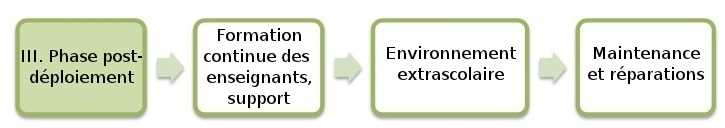
\includegraphics[width=.9\linewidth]{/home/guerry/install/git/OLPC-Deployment--community--guide/images/16_post_deploy_fr.jpg}
\caption{Du post-déploiement à la maintenance/réparation}
\end{figure}

L'implication de la communauté dans le projet est aussi un facteur clé de
sa réussite. À cet effet, de nombreux projets créent des portails Internet
qui sont ouverts aux étudiants, à leurs enseignants et à leur parents afin
que tous puissent partager des informations et voir les progrès des
élèves. De nombreux projets prévoient également des concours intégrant les
XO (ils peuvent être financés par des sponsors privés). D'autres idées
permettant d'impliquer la communauté dans le projet sont disponibles sur
les sites Internet et les portails créés par d'autres projets OLPC dans le
monde.

Chaque projet devrait avoir en parallèle un programme de relations
publiques afin de structurer le support communautaire, développer la
confiance dans le projet et dans ses résultats et comme moyen d'attirer de
nouveaux financements. Bien des projets disposent de programmes
internationaux de relations publiques ; ceux-ci apportent un intérêt
académique au projet local, ce qui entraîne la venue ponctuelle
d'institutions multilatérales intéressées dans les projets sociaux et
éducatifs. À travers son programme de relations publiques, le projet
Ceibal, en Uruguay, est devenu l'un des laboratoires de premier plan dans
le monde au niveau éducatif.

\textbf{Etudes d'évaluation}

\index{Evaluation}

Beaucoup de projets évaluent une première fois leurs étudiants puis les
réévaluent chaque semestre ou année ; les Nations unies évaluent sur une
base semestrielle; les grands projets en général chaque année. L'avantage
des évaluations est le feedback objectif et transparent sur la réussite du
projet ; de plus, beaucoup d'institutions financières multilatérales les
exigent. OLPC laisse au sponsor la décision d'une évaluation mais peut
apporter des ressources pour mettre en oeuvre un programme d'évaluation.
\subsection{Formation et support continus aux enseignants}
\label{sec-10-1}


\index{Formation!Enseignants}
\index{Support!Enseignants}

Les enseignants jouent un rôle clé dans tout déploiement réussi ; au fur et
à mesure qu'ils voient grandir l'enthousiasme de leurs étudiants à
apprendre avec leurs XO, ils sont de plus en plus demandeurs pour leur
propre formation (intégration de Sugar dans le cursus, développement de
cours utilisant les XO. Chaque projet devrait être conçu de façon à
apporter au minimum une journée par mois de formation complémentaire aux
enseignants impliqués dans le projet. Il est aussi à noter que les
formateurs des enseignants auront eux-mêmes besoin d'une formation
ponctuelle d'OLPC afin de renforcer la pédagogie et d'augmenter leurs
compétences.

Une fois la formation initiale des enseignants terminée, l'équipe éducative
locale doit leur apporter des mécanismes de soutien complémentaires afin de
faciliter l'intégration des XO dans la routine des cours; le support fait
en classe ou l'aide apportée à élaborer un plan de cours sont, par exemple,
des stratégies adaptées au domaine scolaire. Des rencontres régulières avec
les enseignants apportent des feedback directs à l'équipe éducative : cela
lui permet de préparer des ateliers complémentaires qui répondent aux
besoins spécifiques des enseignants et étudiants. Ces rencontres sont aussi
l'opportunité pour les enseignants de partager leurs expériences,
d'apprendre de nouvelles stratégies, de préparer des projets
interdisciplinaires et de favoriser des liens scolaires étroits.

Le contenu est un autre domaine sur lequel l'équipe principale a
constamment à travailler : il est en effet primordial que les enseignants
aient accès à des ressources innovatrices et actualisées. À titre
d'exemple, le contenu pourrait être composé de plans de cours, de guides et
de fiches  d'évaluation, d'études de cas, de ressources en ligne et de
blog.
\subsection{Environnement parascolaire}
\label{sec-10-2}


\index{Curriculum}
\index{Parascolaire}

Les programmes parascolaires durant lesquels les enfants peuvent utiliser
leurs XO sont essentiels pour une expérience pédagogique significative.

Quand les enfants sont occupés à utiliser leur XO pour des activités qui
les intéressent et qui sortent des contenus des cours, il leur est possible
d'explorer en toute liberté leurs intérêts tout en développant de nouvelles
compétences technologiques ; ceci leur permet d'utiliser leurs propres
liberté d'expression et créativité et, en conséquence, de développer une
aisance technologique tout en augmentant leur motivation et leur sens des
responsabilités, ce qui amène un impact extraordinaire sur leur vie.

Nous recommandons de concevoir et d'organiser des programmes après les
cours ou durant le week-end, de créer des clubs ou des réunions sur
différents sujets ou activités, dans différentes écoles et communautés. Ces
programmes peuvent inclure des enseignants et des élèves de différents
niveaux ainsi que des partenaires locaux en les faisant participer à une
expérience enrichissante durant laquelle enseignants et élèves créent,
collaborent et partagent projets et idées.

Intégrer la famille à travers les activités offertes par le XO amène les
parents à travailler avec leurs enfants sur des projets directement liés à
leurs centres d'intérêts : c'est enrichissant pour tous ! L'objectif n'est
pas seulement de permettre aux parents de partager connaissances et
expériences avec leurs enfants, mais aussi de comprendre la valeur de
l'apprentissage avec le XO ainsi que son utilité dans le processus
d'apprentissage : ce qui est important pour la viabilité et la durabilité
du projet !
\subsection{Maintenance et réparations}
\label{sec-10-3}


\index{Maintenance}
\index{Réparation}

La réparation des XO peut être traitée de multiples façons. Les trois
méthodes les plus répandues sont les suivantes :

\begin{enumerate}
\item les étudiants réparent eux-mêmes leur XO : des pièces de rechange
   peuvent être envoyées aux écoles sur une base bimensuelle et sur
   commande ;
\item les XO sont réparés par l'atelier local de réparation : cette approche
   offre un apport de travail à la communauté concernée ;
\item les XO sont réparés par des techniciens se rendant dans les écoles sur
   une base bimensuelle pour y effectuer les réparations nécessaires.
\end{enumerate}

Le choix de la méthode de réparation dépend des objectifs éducatifs,
politiques et économiques du sponsor de projet. En ce qui concerne les
réparations, une autre question demeure : qui prend en charge le paiement
des pièces et de la main d'oeuvre ? Certains projets prennent en charge la
première réparation, les suivantes étant à la charge des parents des
enfants concernés ; d'autres projets prennent en charge toutes les
réparations parce que les parents n'ont tout simplement pas les moyens des
les assumer, même lorsque il s'agit de petites sommes. La réglementation
sur les réparations et leur prise en charge doit être expliquée lors de la
présentation initiale du projet à la communauté (destinée aux directeurs
d'école et aux parents).

Le nombre de XO envoyés est majauré de 1 \% par rapport à la commande
initiale. Ces XO supplémentaires sont à disposition pour remplacer
d'éventieuls XO défectueux. Il est important de savoir que les XO
défectueux contiennent des pièces qui peuvent être réutilisées sur d'autres
ordinateurs (comme l'écran, l'antenne WiFi, la carte-mère.)

Les réparations, pour la plupart et y compris le remplacement de la
carte-mère, peuvent être faites sur place à l'aide d'un simple tournevis !
Les enfants peuvent même les effectuer eux-mêmes : c'est un geste et une
responsabilité que nous encourageons ; tout comme l'est la redistibution
locale des pièces de rechange ou encore la création de centres de
réparation locaux.

Si un support d'ordre commercial venait à être arrangé, OLPC ne
l'encouragerait pas pour les raisons suivantes : d'une part, l'augmentation
des coûts, et d'autre part, une dépendance extérieure qui est à éviter.

Si le projet ressent le besoin d'investir dans un support technique, nous
vous encourageons à faire cet investissement localement, la communauté sur
place pouvant être formée aux réparations par notre équipe technique.
\section{Résumé des tâches recommandées}
\label{sec-11}
\subsection{Phase de planification}
\label{sec-11-1}


\begin{itemize}
\item Définir un budget pour : l'achat, l'infrastructure, la connectivité, le
  personnel.
\item Embaucher un responsable de projet et des responsables pour l'équipe
  principale.
\item Choisir les communautés ciblées (écoles, centres).
\item Définir les spécifications du XO.
\end{itemize}
\subsection{Phase de déploiement}
\label{sec-11-2}


\begin{itemize}
\item Embaucher du personnel pour l'équipe principale.
\item Mettre en place une formation pour l'équipe principale avec OLPC.
\item Développer le plan de distribution des ordinateurs.
\item Définir et rassembler des données pour une étude préliminaire.
\item Préparer l'infrastructure et la connectivité (au niveau des écoles et des
  communautés).
\item Organiser et faire des formations pour les enseignants.
\item Distribuer les ordinateurs.
\end{itemize}
\subsection{Phase postdéploiement}
\label{sec-11-3}


\begin{itemize}
\item Définir et mettre en oeuvre une stratégie de support technique pour la
  maintenance et la réparation des ordinateurs.
\item Définir et superviser des environnements d'apprentissage pour le XO :
  formels (à l'école, dans la classe), non-formels (activités
  extra-scolaires) et informels (maison, famille.)
\item Faire le suivi des formations pour les enseignants.
\item Définir et mettre en oeuvre des études d'évaluation (pour l'apprentissage
  des élèves et l'implémentation du projet.)
\end{itemize}
\section{Liens utiles}
\label{sec-12}


\begin{itemize}
\item Site officiel d'OLPC : \href{http://laptop.org}{http://laptop.org}
\item Le wiki d'OLPC : \href{http://wiki.laptop.org}{http://wiki.laptop.org}
\item La version wiki de ce guide de déploiement \href{http://wiki.laptop.org/go/Deployment_Guide}{en anglais}
\item Le manuel Sugar, en page web ou en pdf sur \href{http://en.flossmanuals.net/Sugar}{Flossmanuals}
\item Le forum officiel de la communauté de support d'OLPC
\item La Foire aux Questions : \href{http://wiki.laptop.org/go/Support_FAQ}{http://wiki.laptop.org/go/Support\_FAQ}
\item Le wiki de Sugar Labs, qui fournit l'environnement Sugar et les activités
  qui tournent sur les ordinateurs XO.
\item Le site d'OLPC France : \href{http://olpc-france.org}{http://olpc-france.org}
\end{itemize}
\section{Licence, versions et crédits}
\label{sec-13}
\subsection{Licence}
\label{sec-13-1}


Ce document est sous licence Creative Commons \href{http://creativecommons.org/licenses/by/3.0/}{CC BY 3.0}.  Il est permis à
quiconque d'utiliser ce document et d'en produire des versions dérivées
tant que la source et l'auteur original (One Laptop Per Child) sont cités.
\subsection{Versions}
\label{sec-13-2}


La version anglaise de ce document est disponible \href{http://wiki.laptop.org/images/1/1c/OLPC_Deployment_Guide_2011.pdf}{au format PDF} et \href{http://wiki.laptop.org/go/Deployment_Guide_2011}{en version Wiki} sur le site d'OLPC.

Les sources pour la traduction sont disponibles via \href{https://github.com/bzg/OLPC-Deployment--community--guide}{ce dépôt git}, qui
contient le fichier original (PDF), une version en \href{http://fr.wikipedia.org/wiki/OpenDocument}{Open Document Format} et
une version texte utilisant le format \href{http://orgmode.org}{Org-mode}.  Les conversions en \texttt{.odt}
\texttt{HTML} et \texttt{PDF} ont été effectuées via org-mode.

Le site d'OLPC France héberge \href{http://olpc-france.org/guide-deploiement/olpc-guide-deploiement.pdf}{une version PDF} et une \href{http://olpc-france.org/guide-deploiement/olpc-guide-deploiement.html}{version HTML}.  Il
existe aussi une \href{http://olpc-france.org/guide-deploiement/index.html}{version en ligne} que nous vous engageons à \emph{commenter}:
posez-y toutes les questions que vous avez sur les déploiments OLPC ou 
sur le guide lui-même, OLPC France essaiera d'y répondre.
\subsection{Crédits}
\label{sec-13-3}


La traduction française a été faite par OLPC France entre septembre et
novembre 2011.  Merci aux membres d'OLPC France qui y ont contribué :

\begin{itemize}
\item Cécile Wyler Roulet
\item Kévin Raymond
\item Pierre Varly
\item Bastien Guerry
\end{itemize}

\end{document}
